\documentclass{chi-ext}
% Please be sure that you have the dependencies (i.e., additional LaTeX packages) to compile this example.
% See http://personales.upv.es/luileito/chiext/

\usepackage{wrapfig}


\title{Portrait Pigeon: An Interactive Photo Messaging Wall for Seniors}

\numberofauthors{3}
% Notice how author names are alternately typesetted to appear ordered in 2-column format;
% i.e., the first 4 autors on the first column and the other 4 auhors on the second column.
% Actually, it's up to you to strictly adhere to this author notation.
\author{
  \alignauthor{
  	\textbf{Robin N. Brewer}\\
  	\affaddr{Northwestern University}\\
  	\affaddr{2240 Campus Drive}\\
  	\affaddr{Evanston, IL 60208 USA}\\
  	\email{rnbrewer@u.northwestern.edu}
  }
  \vfil
  \alignauthor{
  	\textbf{Moritz Gellner}\\
  	\affaddr{Northwestern University}\\
  	\affaddr{2240 Campus Drive}\\
  	\affaddr{Evanston, IL 60208 USA}\\
  	\email{moritzgellner2014@u.northwestern.edu}
  }
  \vfil
  \alignauthor{
  	\textbf{Anne Marie Piper}\\
  	\affaddr{Northwestern University}\\
  	\affaddr{2240 Campus Drive}\\
  	\affaddr{Evanston, IL 60208 USA}\\
  	\email{ampiper@northwestern.edu}
  }
}

% Paper metadata (use plain text, for PDF inclusion and later re-using, if desired)
\def\plaintitle{Portrait Pigeon An Interactive Photo Messaging Wall for Seniors}
\def\plainauthor{Robin N. Brewer}
\def\plainkeywords{Older adults, gesture input, lightweight communication}
\def\plaingeneralterms{Design, Human Factors}

\hypersetup{
  % Your metadata go here
  pdftitle={\plaintitle},
  pdfauthor={\plainauthor},  
  pdfkeywords={\plainkeywords},
  pdfsubject={\plaingeneralterms},
  % Quick access to color overriding:
  %citecolor=black,
  %linkcolor=black,
  %menucolor=black,
  %urlcolor=black,
}

\usepackage{graphicx}   % for EPS use the graphics package instead
\usepackage{balance}    % useful for balancing the last columns
\usepackage{bibspacing} % save vertical space in references


\begin{document}

\maketitle

\begin{abstract}
Considerable research has studied online communication for older adults. For some seniors, age-related disability presents barriers to using computers and going online. For others, lack of experience or lack of interest deters them from keeping in touch using modern communication platforms such as social media sites. Physical communication artifacts, such as printed photos, support important forms of offline communication for older adults, and we examine how physical photos can be augmented to facilitate lightweight online social communication. This approach embeds online messaging into a familiar and culturally-relevant artifact, \emph{physical photos}. This paper presents Portrait Pigeon, a ubiquitous lightweight messaging platform for seniors that integrates in-home photo displays into online communication.
\end{abstract}

\keywords{\plainkeywords}

\category{H.5.m}{Information interfaces and presentation (e.g., HCI)}{Miscellaneous}. 

%\terms{\plaingeneralterms}


% =============================================================================
\section{Introduction}
% =============================================================================
Age-related disability and chronic health conditions make it more difficult for older adults to use computers and go online~\cite{pew:2014}. For some older adults, lack of interest or relevance may deter them staying in touch online~\cite{sundar:2011,Pew2012}. Embedding online interaction in everyday artifacts is a rich area for ubiquitous computing design. This approach stands to support older users who are less familiar with going online while integrating online communication into one's daily routines and living environment. Our work builds on prior research of older adults' values around storing and revisiting non-digital photographs \cite{Swan2008}. Portrait Pigeon allows older adults to interact with physical walls of photos through gesture-based input and, based on relative body movements in front of the photo wall, sends lightweight online messages to the people in the physical photos.

Prior work examines the social practices of viewing and sharing physical photographs~\cite{lindley:2009,Swan2008}. Augmenting photo frames is a common approach to designing social experiences for older adults~(e.g., \cite{arreola:2014,mynatt:2001}). We extend this idea to include walls of physical photos, which leverage the semi-permanent nature of these photo displays~\cite{Swan2008}. Portrait Pigeon integrates static physical photos with dynamic online interaction through a flexible and customizable gesture-based interface, enabling a new form of lightweight communication for older adults~\cite{lindley:2012}.

Transforming static walls, tables, and objects into interactive surfaces is often accomplished through the use of a depth camera (e.g.,~\cite{Corsten2013,Wilson2010}), and we apply this technique to photo displays on physical walls. Through the design and development of Portrait Pigeon, we examine: 1) how to tailor whole-body, gesture interactions to older adults with various disabilities, 2) flexible linking of different modes of lightweight messaging (e.g., e-mail, voice, social media), and 3) various feedback mechanisms. 


%We simplify the training of the interactive environment through a simple interface where seniors map locations of their natural environment to the platform account (i.e. email address or Twitter handle) of the person in the picture frame. Also, we extend re-purposing of objects by focusing on the use of photo frames for email messaging through text and voice. The contributions of this work are 1) tailoring interaction for older adults with various disabilities, 2) linking different modes of lightweight messaging, and 3) prototyping feedback mechanisms. 

%%\begin{wrapfigure}{l}{3cm}
%\begin{figure}
%  \begin{center}
%  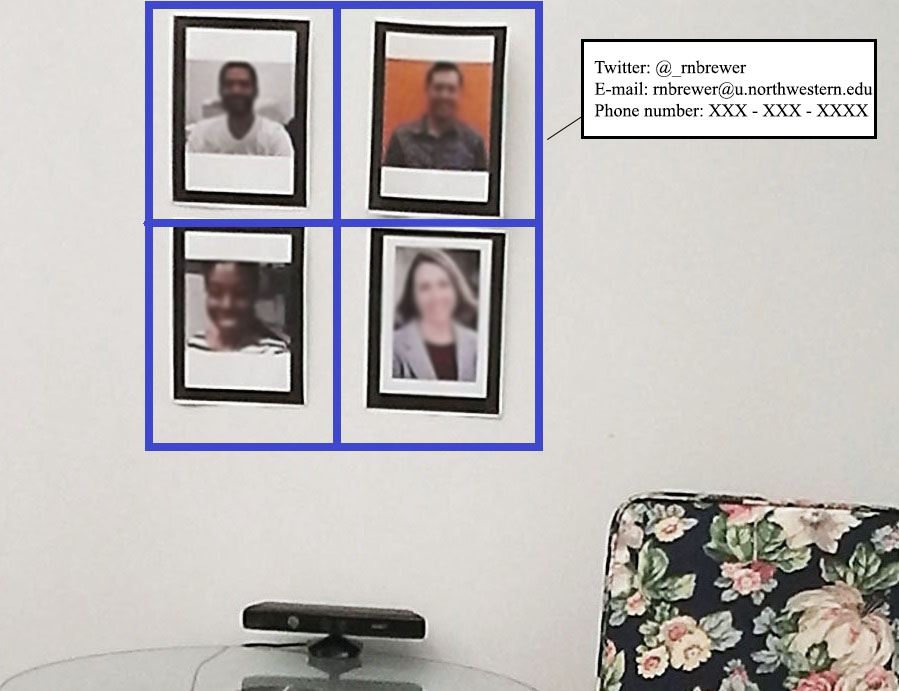
\includegraphics[width=\columnwidth]{photo-chair-crop.png}
%  \caption{Gesturing toward a photo initiates an online message to the person in the photo.}
%  \label{fig:currgrid}
%  \end{center}  
%\end{figure}
%%\end{wrapfigure}

% =============================================================================
\section{Portrait Pigeon}
% =============================================================================
Portrait Pigeon uses a Microsoft Kinect, the SimpleOpenNI library, and Processing for interacting with physical photos. The Kinect is positioned on the same wall as the photos, facing the user (Figure 1).

\subsection{Customizing body-based interaction for older adults}
Gestures are detected as \emph{relative movements} targeted towards quadrants of the photo wall by calculating arm movement relative to the user's torso. For example, if a picture is in the top left quadrant, a gesture is recognized when a hand (right or left) is placed above and to the left of their torso. The relative positioning and recognition of gestures can be customized to an individual's physical abilities. For example, target selection is initially based on hand position relative to the hip or waist for standing individuals, but for people with more limited range of motion or who use a wheelchair, selection can be based on hand movement relative to the torso or shoulder. This customization is particularly important for older adults who have highly diverse physical abilities and could be tailored specifically to users in wheelchairs~\cite{gerling:2013}. 

\begin{figure}
    \centering
    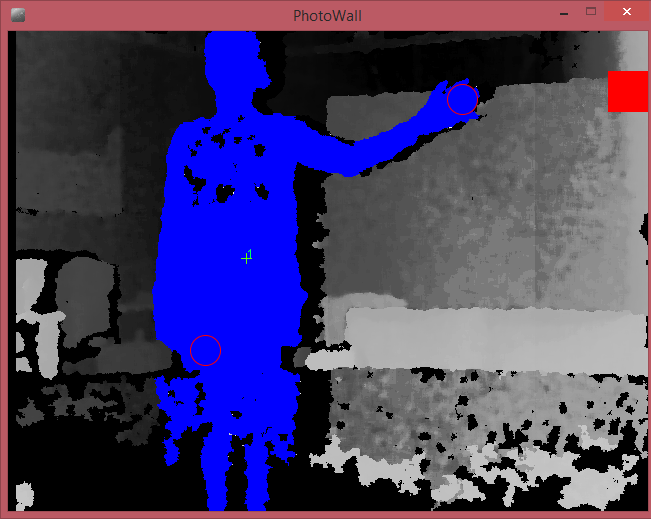
\includegraphics[width=0.22\textwidth]{depthtracking.png} 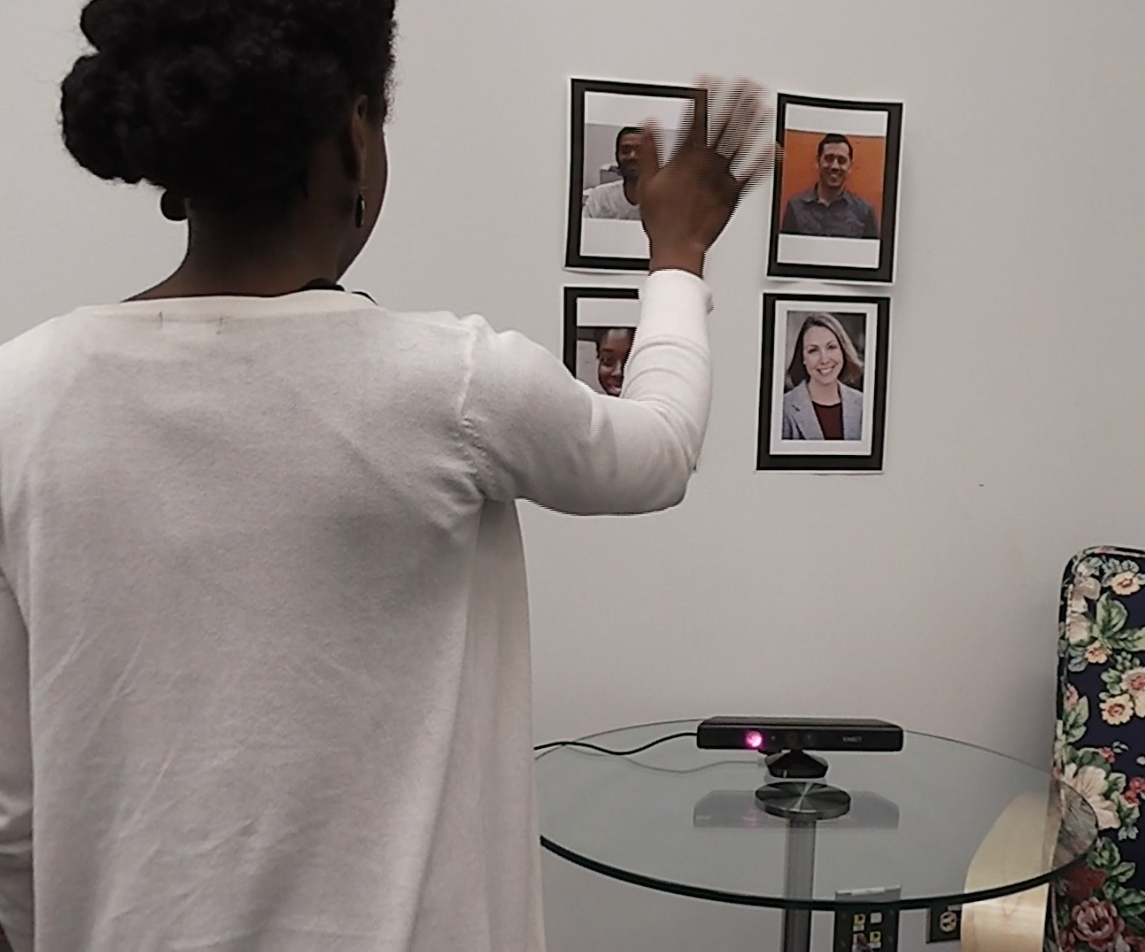
\includegraphics[width=0.2\textwidth]{backwallshot.png}
	\texttt{twitter: @johndoe \\*
	email: johndoe@johndoe.com \\*}    
    \caption{The user can toggle between different platforms such as posting a tweet or sending an e-mail message. Upon target placement, the message is sent.}
	 \label{fig:tracking}
\end{figure}

\subsection{Flexible integration of lightweight messaging}
% -----------------------------------------------------------------------------
Portrait Pigeon can be configured to send various predefined text-based e-mail messages, Twitter posts, or voice-recorded messages, which can be sent as an e-mail attachment. As a proof-of-concept, we have explored pre-set e-mail messages (e.g., ``I am thinking of you.'') which are sent to the person in the photo when a user gestures towards that person's picture on the wall. Our initial focus has been on sending lightweight messages through e-mail given it's pervasiveness with older adults \cite{Pew2012} but also because accessing and using graphical e-mail accounts can become increasingly difficult for older adults with low vision or mobility impairments, providing a new way of maintaining e-mail communication. Portrait Pigeon may also benefit older adults with cognitive disabilities, because it draws on the social practice of acknowledging someone with gesture (e.g. a wave hello) and initiates communication with them online (e.g. sending an email message) without the need for logging in or managing an online e-mail account. The assignment of message type and content is flexible and enables integration of multiple messaging platforms (e.g., Facebook, Twitter, text messaging), although this currently needs to be set up and configured by a caregiver.

% =============================================================================
\subsection{Exploring feedback mechanisms}
% =============================================================================
It is important to notify older adults that a message was successfully sent and to help users avoid accidental activation. Our current system uses audio (i.e., ~a chime) to inform the user that an e-mail message has been sent. We are improving our prototype to include visual feedback projected onto the wall using a short-throw projector (e.g.,~\cite{Wilson2010}), and this multimodal visual-auditory feedback will be important for older adults with hearing loss but could also provide subtle ambient cues when a user is in range of the interactive photo wall. Additionally, we are exploring the use of visual cues to guide users to successful selection of a photo on a wall, which will be important to prototype and test with photo walls that include multiple, small targets. Real-time visual feedback when selecting among multiple small targets is particularly important given the use of relative body positioning, whereas absolute positioning (i.e.,~reaching to touch directly on a photo) may have greater precision for some users but be too difficult for others with physical disabilities who cannot reach the wall. %Using the Kinect's depth sensor, we are able to approximate the position on the wall that a user is currently pointing at and project a mark onto that spot to make the user aware of relative positioning(\autoref{fig:depthdiagram}). This would make the system more interactive and intuitive to use, which is important to engage older adults that are less inclined to experiment with new technology.

\section{Pilot Testing with Older Adults}
As part of our broader research, we have conducted field observations in local retirement communities over the past year, and the idea for Portrait Pigeon emerged from this extensive qualitative research. In these communities, we observe numerous instances of photo displays that could be augmented and connected online to enable lightweight messaging. Beyond photo walls in an individual's room, communities display walls of photos of staff members, mailboxes with residents' names, and bulletin boards with photos from recent events. To test the initial concept of Portrait Pigeon, we installed our system in one drop-in computer room at an assisted living community. We instrumented a wall of photos of community staff as a way to send ``Thank You'' messages to staff members. Three researchers observed casual use of the photo wall by older adults and other staff in the computer room. Several older adults were hesitant to use Portrait Pigeon fearing it may take too much time or that they didn't have a message to send to the staff in the photos. Others successfully sent messages to staff using the system. Although this feature was not yet enabled, one user expected to be able to record and send an audio message, as he gestured toward a message recipient and began speaking his message after the `message sent' chime played. Across these users we noted issues of Kinect placement, range of motion limitations, and challenges with wheelchair use that will inform future iterations of this prototype. 

%Based on feedback from this initial testing, we are incorporating visual feedback to halo a person's hand to guide them on how to reach the target. Based on the existing coordinates of a user's shoulder and skeleton, we are able to calculate and recognize the angle of a person's hand and where it is pointing. We are also taking advantage of the embedded microphone in the Kinect that could record voice messages of users and email those to the target person in the photo. 



% =============================================================================
\section{Conclusion and Future Work}
% =============================================================================
Portrait Pigeon supports lightweight communication with family and friends through physical photo displays, lowering the barrier of entry for older adults who have difficulty using computers or are not familiar accessing the internet. This approach has the potential to integrate older adults into online communication platforms (e.g. Facebook, Twitter) in a way that leverages their existing practices and experiences with physical photos.  Given the wide range in abilities and communication needs of older adults, we highlight the need for further exploration of customized body-based input, integration with a variety of messaging platforms, and multimodal feedback. In the future we will expand the system to incorporate reciprocal communication where people tagged in the portraits can send messages to the physical photo wall (i.e.,~a projected speech bubble appears by the frame).	

%\subsection{Ease of Set-up - CLARIFY since you don't do this yet}
%An important design challenge is creating a setup that is simple for older adults and their families to initialize. In order to know where the photos are located, Portrait Pigeon must first obtain a picture of the environment. Prior to sending the first message, users must upload a picture of their photo wall and tag people in the photos (\autoref{currgrid}). If there is more than one person in the photo, it is up to the user to define which person they would want to send a message to. Also if a picture is moved, the system allows for easy reconfiguration of the wall setup. This can also be extended to pictures in frames and not on walls as long as the frames are on the same side of the wall as the Kinect. While we recognize this may be a limitation for older adults without a digital camera or cell phone, additional depth-sensors would allow us to replace this manual setup with an automatic setup, where a second Kinect would capture the location and content of pictures on the photo wall. Furthermore, computer vision could be used to implement automatic facial recognition so that Portrait Pigeon could automatically associate the framed pictures with stored contact information. This would reduce its reliance on such a rigid coordinate system in which pictures can be placed; instead, contacts could be mapped to arbitrary and more precise spatial areas.


\balance
\bibliographystyle{acm-sigchi}
\bibliography{sample}

\end{document}